%%%%%%%%%%%%%%%%%%%%%%%%%%%%%%%%%%%%%%%%%
% Programming/Coding Assignment
% LaTeX Template
%
% This template has been downloaded from:
% http://www.latextemplates.com
%
% Original author:
% Ted Pavlic (http://www.tedpavlic.com)
%
% Note:
% The \lipsum[#] commands throughout this template generate dummy text
% to fill the template out. These commands should all be removed when 
% writing assignment content.
%
% This template uses a Perl script as an example snippet of code, most other
% languages are also usable. Configure them in the "CODE INCLUSION 
% CONFIGURATION" section.
%
%Assignment 2
%Author Zetan
%%%%%%%%%%%%%%%%%%%%%%%%%%%%%%%%%%%%%%%%%

%----------------------------------------------------------------------------------------
%	PACKAGES AND OTHER DOCUMENT CONFIGURATIONS
%----------------------------------------------------------------------------------------

\documentclass{article}

\usepackage{fancyhdr} % Required for custom headers
\usepackage{lastpage} % Required to determine the last page for the footer
\usepackage{extramarks} % Required for headers and footers
\usepackage[usenames,dvipsnames]{color} % Required for custom colors
\usepackage{graphicx} % Required to insert images
\usepackage{listings} % Required for insertion of code
\usepackage{courier} % Required for the courier font
\usepackage{multirow}
\usepackage{listings,multicol}

\usepackage{url}

% Margins
\topmargin=-0.45in
\evensidemargin=0in
\oddsidemargin=0in
\textwidth=6.5in
\textheight=9.0in
\headsep=0.25in

\linespread{1.1} % Line spacing

% Set up the header and footer
\pagestyle{fancy}
\lhead{\hmwkAuthorName} % Top left header
\chead{\hmwkClass\ (\hmwkClassInstructor\ \hmwkClassTime): \hmwkTitle} % Top center head
\rhead{\firstxmark} % Top right header
\lfoot{\lastxmark} % Bottom left footer
\cfoot{} % Bottom center footer
\rfoot{Page\ \thepage\ of\ \protect\pageref{LastPage}} % Bottom right footer
\renewcommand\headrulewidth{0.4pt} % Size of the header rule
\renewcommand\footrulewidth{0.4pt} % Size of the footer rule

\setlength\parindent{0pt} % Removes all indentation from paragraphs

%----------------------------------------------------------------------------------------
%	CODE INCLUSION CONFIGURATION
%----------------------------------------------------------------------------------------

\definecolor{MyDarkGreen}{rgb}{0.0,0.4,0.0} % This is the color used for comments
\lstloadlanguages{Python} % Load python syntax for listings, for a list of other languagesftp://ftp.tex.ac.uk/tex-archive/macros/latex/contrib/listings/listings.pdf supported see: 
\lstset{
        frame=single, % Single frame around code
        basicstyle=\small\ttfamily, % Use small true type font
        keywordstyle=[1]\color{Blue}\bf, % python functions bold and blue
        keywordstyle=[2]\color{Purple}, % python function arguments purple
        keywordstyle=[3]\color{Blue}\underbar, % Custom functions underlined and blue
        identifierstyle=, % Nothing special about identifiers                                         
        commentstyle=\usefont{T1}{pcr}{m}{sl}\color{MyDarkGreen}\small, % Comments small dark green courier font
        stringstyle=\color{Purple}, % Strings are purple
        showstringspaces=false, % Don't put marks in string spaces
        tabsize=5, % 5 spaces per tab
        breaklines=true,
        %
        % Put standard python functions not included in the default language here
        morekeywords={rand},
        %
        % Put python function parameters here
        morekeywords=[2]{on, off, interp},
        %
        % Put user defined functions here
        morekeywords=[3]{test},
       	%
        morecomment=[l][\color{Blue}]{...}, % Line continuation (...) like blue comment
        numbers=left, % Line numbers on left
        firstnumber=1, % Line numbers start with line 1
        numberstyle=\tiny\color{Blue}, % Line numbers are blue and small
        stepnumber=5 % Line numbers go in steps of 5
}

% Creates a new command to include a pyton script, the first parameter is the filename of the script (without .py), the second parameter is the caption
\newcommand{\pythonscript}[2]{
\begin{itemize}
\item[]\lstinputlisting[language=python,caption=#2,label=#1]{#1.py}
\end{itemize}
}
% Creates a new command to include a shell script, the first parameter is the filename of the script (without .sh), the second parameter is the caption
\newcommand{\shellscript}[2]{
\begin{itemize}
\item[]\lstinputlisting[language=bash,caption=#2,label=#1]{#1.sh}
\end{itemize}
}
% Creates a new command to include a R script, the first parameter is the filename of the script (without .R), the second parameter is the caption
\newcommand{\Rscript}[2]{
\begin{itemize}
\item[]\lstinputlisting[language=R,caption=#2,label=#1]{#1.R}
\end{itemize}
}
%----------------------------------------------------------------------------------------
%	DOCUMENT STRUCTURE COMMANDS
%	Skip this unless you know what you're doing
%----------------------------------------------------------------------------------------

% Header and footer for when a page split occurs within a problem environment
\newcommand{\enterProblemHeader}[1]{
\nobreak\extramarks{#1}{#1 continued on next page\ldots}\nobreak
\nobreak\extramarks{#1 (continued)}{#1 continued on next page\ldots}\nobreak
}

% Header and footer for when a page split occurs between problem environments
\newcommand{\exitProblemHeader}[1]{
\nobreak\extramarks{#1 (continued)}{#1 continued on next page\ldots}\nobreak
\nobreak\extramarks{#1}{}\nobreak
}

\setcounter{secnumdepth}{0} % Removes default section numbers
\newcounter{homeworkProblemCounter} % Creates a counter to keep track of the number of problems

\newcommand{\homeworkProblemName}{}
\newenvironment{homeworkProblem}[1][Problem \arabic{homeworkProblemCounter}]{ % Makes a new environment called homeworkProblem which takes 1 argument (custom name) but the default is "Problem #"
\stepcounter{homeworkProblemCounter} % Increase counter for number of problems
\renewcommand{\homeworkProblemName}{#1} % Assign \homeworkProblemName the name of the problem
\section{\homeworkProblemName} % Make a section in the document with the custom problem count
\enterProblemHeader{\homeworkProblemName} % Header and footer within the environment
}{
\exitProblemHeader{\homeworkProblemName} % Header and footer after the environment
}

\newcommand{\problemAnswer}[1]{ % Defines the problem answer command with the content as the only argument
\noindent\framebox[\columnwidth][c]{\begin{minipage}{0.98\columnwidth}#1\end{minipage}} % Makes the box around the problem answer and puts the content inside
}

\newcommand{\homeworkSectionName}{}
\newenvironment{homeworkSection}[1]{ % New environment for sections within homework problems, takes 1 argument - the name of the section
\renewcommand{\homeworkSectionName}{#1} % Assign \homeworkSectionName to the name of the section from the environment argument
\subsection{\homeworkSectionName} % Make a subsection with the custom name of the subsection
\enterProblemHeader{\homeworkProblemName\ [\homeworkSectionName]} % Header and footer within the environment
}{
\enterProblemHeader{\homeworkProblemName} % Header and footer after the environment
}

%----------------------------------------------------------------------------------------
%	NAME AND CLASS SECTION
%----------------------------------------------------------------------------------------

\newcommand{\hmwkTitle}{Assignment\ \#4} % Assignment title
\newcommand{\hmwkDueDate}{Thursday,\ February\ 25,\ 2016} % Due date
\newcommand{\hmwkClass}{Web Science\ cs532} % Course/class
\newcommand{\hmwkClassTime}{4:20pm} % Class/lecture time
\newcommand{\hmwkClassInstructor}{Dr.Michael.L.Nelson} % Teacher/lecturer
\newcommand{\hmwkAuthorName}{Zetan Li} % Your name

%----------------------------------------------------------------------------------------
%	TITLE PAGE
%----------------------------------------------------------------------------------------

\title{
\vspace{2in}
\textmd{\textbf{\hmwkClass:\ \hmwkTitle}}\\
\normalsize\vspace{0.1in}\small{Due\ on\ \hmwkDueDate}\\
\vspace{0.1in}\large{\textit{\hmwkClassInstructor\ \hmwkClassTime}}
\vspace{3in}
}

\author{\textbf{\hmwkAuthorName}}
\date{} % Insert date here if you want it to appear below your name

%----------------------------------------------------------------------------------------

\begin{document}

\maketitle

%----------------------------------------------------------------------------------------
%	TABLE OF CONTENTS
%----------------------------------------------------------------------------------------

%\setcounter{tocdepth}{1} % Uncomment this line if you don't want subsections listed in the ToC

\newpage
\tableofcontents
\newpage

%----------------------------------------------------------------------------------------
%	PROBLEM 1
%----------------------------------------------------------------------------------------

% To have just one problem per page, simply put a \clearpage after each problem

\begin{homeworkProblem}
Determine if the friendship paradox holds for my Facebook
account.* Compute the mean, standard deviation, and median of the
number of friends that my friends have.  Create a graph of the
number of friends (y-axis) and the friends themselves, sorted by
number of friends (x-axis).  (The friends don't need to be labeled
on the x-axis: just f1, f2, f3, ... fn.)  Do include me in the graph
and label me accordingly.\\
\\
* = This used to be more interesting when you could more easily download
your friend's friends data from Facebook.  Facebook now requires each
friend to approve this operation, effectively making it impossible.\\
\\
I will email to the list the XML file that contains my Facebook
friendship graph ca. Oct, 2013.  The interesting part of the file looks
like this (for 1 friend):\\
\begin{lstlisting}[frame=none]
 <node id="Johan_Bollen_1448621116">
        <data key="Label">Johan Bollen</data>
        <data key="uid"><![CDATA[1448621116]]></data>
        <data key="name"><![CDATA[Johan Bollen]]></data>
        <data key="mutual_friend_count"><![CDATA[37]]></data>
        <data key="friend_count"><![CDATA[420]]></data>
</node>
 \end{lstlisting}

It is in GraphML format: \url{http://graphml.graphdrawing.org/}\\
\centerline{SOLUTION}
First, we should able to parse the graphML. In python, we can use pygraphml to parse the file.
Note that the pygraphml doesn't have any exception handlers, so any missing of keys or values will trigger the
exception and interrupt the parsing.\\
\\
And because of the poor documentation of pygraphml, I have to look into source file to get the idea of which function
to use, in order to retrieve the nodes attribute. Then I find in node.py, there's an member function called nodes(), which can be use to 
get all nodes information without any searching or matching work, because the ID field will trigger the exception for some node's 
ID is 0.\\
\pythonscript{p1}{Python script to parse and sort the number of friends}
From the result, overall statistics are:\\
standard deviation : 369.50\\
mean : 357.73\\
median : 259.00\\
As for the graph, despite the regular dot plot, we have to label the Micheal Nelson in the graph. To add this additional mark, we have to use abline in R, and conceal the regular x-axis labels. Just show the first and last label on the x-axis.\cite{plot}
\Rscript{p1}{R script to plot the facebook friends count}
Below is the graph of friends count.\\
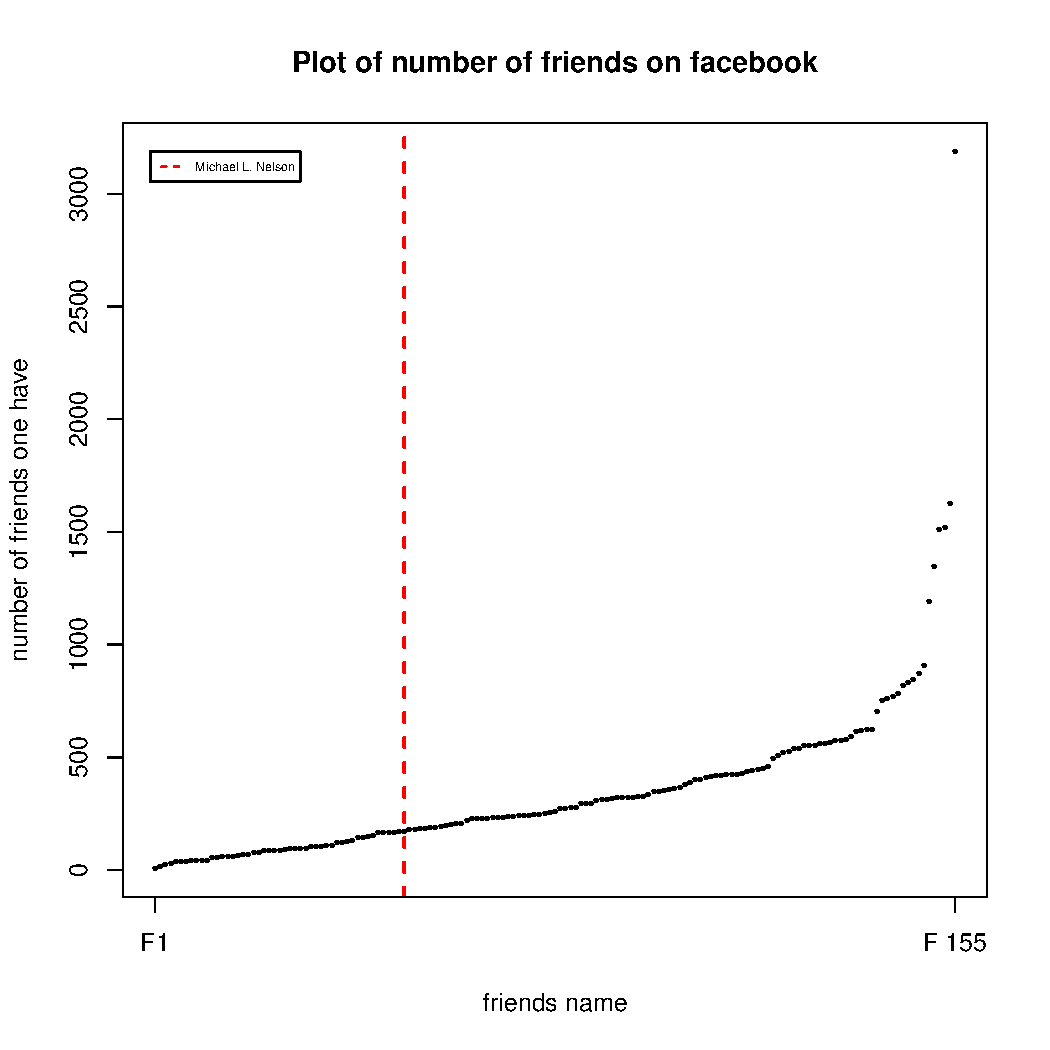
\includegraphics{facebook_plot}
\newpage
Then, as we all know during the discussion, some nodes don't have ``friends\_count'', those nodes have to be dropped. The dropped data is displayed below:
\begin{lstlisting}[ multicols=2,breaklines=true]
ID: 14
mutual_friend_count : 2
Label : James Florance
uid : 501351702
name : James Florance
label : James_Florance_501351702

ID: 31
mutual_friend_count : 0
Label : Joy Gooden
uid : 580143423
name : Joy Gooden
label : Joy_Gooden_580143423

ID: 52
mutual_friend_count : 8
Label : Kim Beveridge
uid : 662936475
name : Kim Beveridge
label : Kim_Beveridge_662936475

ID: 53
mutual_friend_count : 11
Label : Alfredo Sánchez
uid : 667415071
name : Alfredo Sánchez
label : Alfredo_Sánchez_667415071

ID: 60
mutual_friend_count : 19
Label : Sarah Shreeves
uid : 700331809
name : Sarah Shreeves
label : Sarah_Shreeves_700331809

ID: 88
mutual_friend_count : 1
Label : Sally Mauck
uid : 1243862786
name : Sally Mauck
label : Sally_Mauck_1243862786

ID: 96
mutual_friend_count : 0
Label : Dan Swaney
uid : 1321960327
name : Dan Swaney
label : Dan_Swaney_1321960327

ID: 118
mutual_friend_count : 3
Label : Robert Gordeaux
uid : 1580113991
name : Robert Gordeaux
label : Robert_Gordeaux_1580113991

ID: 122
mutual_friend_count : 2
Label : Joseph Kaplan
uid : 1623901873
name : Joseph Kaplan
label : Joseph_Kaplan_1623901873

ID: 133
mutual_friend_count : 17
Label : Michael Milner
uid : 100000008814265
name : Michael Milner
label : Michael_Milner_100000008814265

ID: 134
mutual_friend_count : 3
Label : Catherine Kemble Cronin
uid : 100000016520821
name : Catherine Kemble Cronin
label : Catherine_Kemble_Cronin_100000016520821

\end{lstlisting}
From the graph, we can see most friends are have more friends than you (the mark of Michael, with 165 friends , is closer to the left). So the friendship paradox is true for Michael's facebook account.
\newpage
\end{homeworkProblem}
\pagebreak
%----------------------------------------------------------------------------------------
%	PROBLEM 2
%----------------------------------------------------------------------------------------
\begin{homeworkProblem}
Determine if the friendship paradox holds for your Twitter account.
Since Twitter is a directed graph, use ``followers" as value you measure
(i.e., ``do your followers have more followers than you?").\\
\\
Generate the same graph as in question \#1, and calcuate the same 
mean, standard deviation, and median values.\\
\\
For the Twitter 1.1 API to help gather this data, see:\\
\\
\url{https://dev.twitter.com/docs/api/1.1/get/followers/list}\\
\\
If you do not have followers on Twitter (or don't have more than 50),
then use my twitter account ``phonedude\_mln".\\
\centerline{SOLUTION}
As we already did the similar thing with facebook. This time we just have to find the twitter API, invoke them to get the follower count, and plot the graph by same mechanism.\\
\\
Note that twitter api limits the number of requests to 15 times every 15 minutes. If we are going to fetch the follower data one by one, it most like we will exceed the rate limit and have to wait another 15 minutes for next query.\\
\\
Luckily we can use follower/list api to fetch at most 200 follower information a time. So it only require 3 queries to get the information of around 500 followers of Michael Nelson. (My twitter account is brand new with only 2 I-don't-know-who-she-is followers, so I choose to do the statistics with Michael's account)\\
\\
The statistics of the twitter follower is (in Feb 24,2016):\\
standard deviation : 4140\\
mean : 1042\\
median : 255\\
\pythonscript{p2}{Python script to get the follower's follower information}
Then we are going to do the same thing as we did in problem 1 to plot the graph.
\Rscript{p2}{R script to plot the graph of twitter followers}
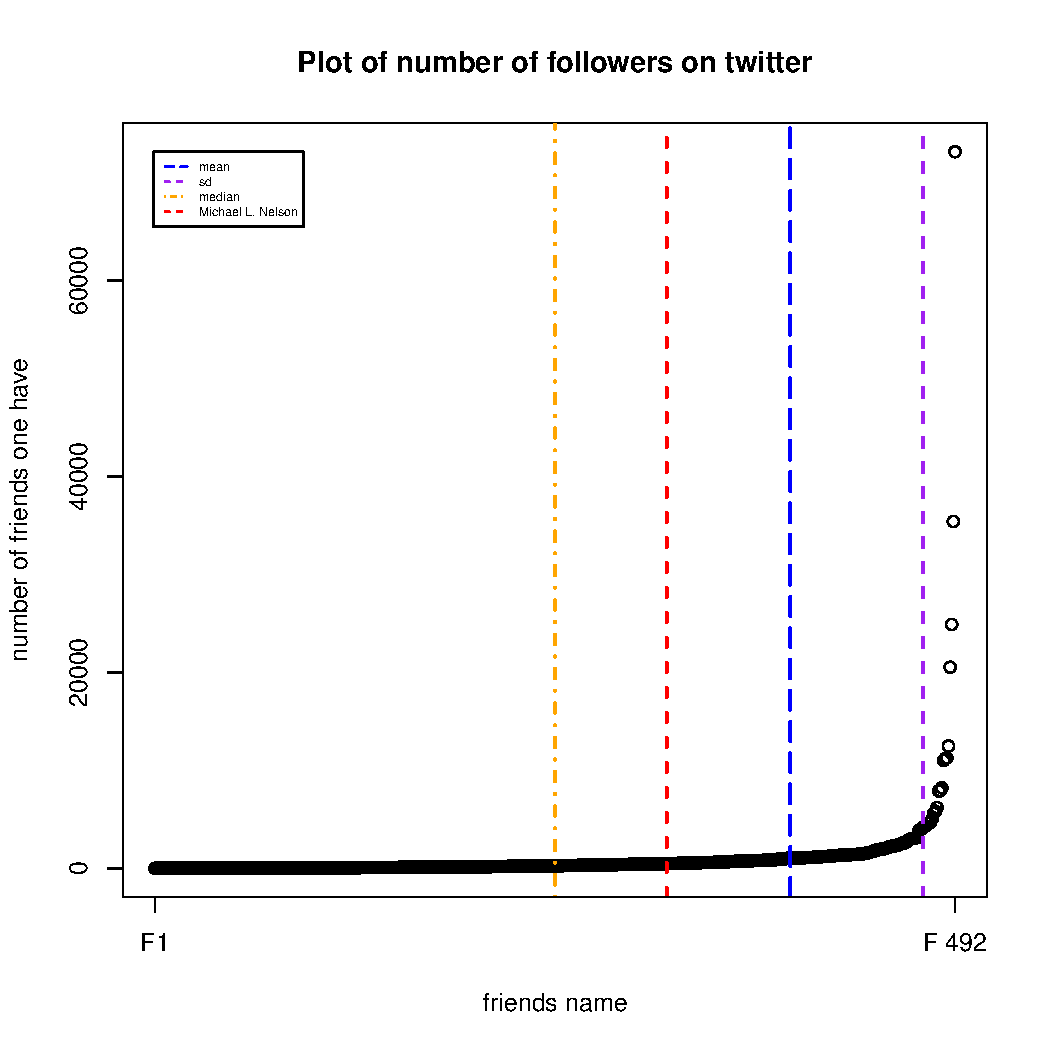
\includegraphics{twitter_plot}
Though this time the mark is rightward a little bit, but there's still many followers who have more followers than Michael does. So the friendship paradox is true here as well.
\end{homeworkProblem}
\bibliographystyle{plain}
\bibliography{ref}
\end{document}